\documentclass[a4paper]{article}  %>>> use for US letter paper
\usepackage[]{graphicx}
\usepackage{url}
\usepackage[colorlinks = true, linkcolor={black},urlcolor={black}]{hyperref}
\pdfforcepagebox=5
\renewcommand{\baselinestretch}{1.25}   %>>> 1.65 for double spacing, 1.25 for 1.5 spacing 
%\usepackage{newcent}
%\usepackage{pslatex} %per avere i font con migliore qualità
% Here we include packages for better formatting and output quality
\usepackage{microtype}
\usepackage{booktabs}
\usepackage{amsmath}
\usepackage[ruled]{algorithm2e} %for pseudo code
\title{Measurements of the time-lag of Optotrak system}

\author{Carlo Nicolini, Robert Volcic}
%>>>> Further information about the authors, other than their 
%  institution and addresses, should be included as a footnote, 
%  which is facilitated by the \authorinfo{} command.

\begin{document}
\maketitle 
\section{Measurement method}
We measured the time-lag with the method described in Swindell. We used a rotational motor and a rod to stick a marker on it and see the angular displacement from real marker to a corrispondend light point on the display.
We rotated the rotor at a speed of $\omega = 1/6$ rpm, equivalent to $\omega = 60^\circ/s$. The time lag $\Delta t$ accumulated in the whole process, from data acquisition to display, is then simply obtained by the relation $\Delta t = \Delta \theta / \omega$. The $\Delta \theta$ were measured manually with ImageJ software.

We took $N=20$ measures of the angular distance between the marker infrared emitting diode and a corrispondent white dot with size $8\times 8$ pixels, on a $1024 \times 768$ display. The marker was rotating on the focal plane, thus eliminating the parallax error to our best possibilities.
We took the photos with a Nikon D90, resolution $3216 \times 2136$, ISO 6400, F-number $4.5$, Exposure time $1/100$, focal length $38$ mm.
We measured the angles with the camera, calibrated with the center of projection made to correspond to the camera CCD sensor center and frontoparallel to the center of rotation. 

Angles were extracted using a manual procedure with ImageJ software. The error bars are the size in angle of the displayed point.

\begin{table}[htb!]\label{tab:table_exp_1}
\centering
\begin{tabular}{|l|l|r|} \hline
$i$ & $\Delta \theta $ [deg] & $\sigma_{\Delta \theta}$ [deg] \\
\hline 
1 & 0.80 & 1.07 \\ \hline 
2 & 2.06 & 0.94 \\ \hline 
3 & 2.15 & 1.22 \\ \hline
4 & 2.26 & 1.25 \\ \hline
5 & 1.80 & 1.25 \\ \hline
6 & 1.80 & 1.21 \\ \hline
7 & 1.44 & 1.02 \\ \hline
8 & 1.67 & 1.08 \\ \hline
9 & 1.96 & 1.05 \\ \hline
10 & 1.67 & 1.15 \\
\hline
\end{tabular}
\begin{tabular}{|l|l|r|} \hline
$i$ & $\Delta \theta$ [deg] & $\sigma_{\Delta \theta}$ [deg]\\
\hline 
11 & 1.90 & 1.06 \\  \hline
12 & 1.10 & 1.16 \\  \hline
13 & 0.94 & 1.11 \\ \hline
14 & 1.70 & 0.95 \\ \hline
15 & 2.40 & 1.01 \\ \hline
16 & 1.90 & 1.17 \\ \hline
17 & 1.70 & 1.15 \\ \hline
18 & 1.49 & 1.14 \\ \hline
19 & 1.11 & 1.03 \\ \hline
20 & 0.41 & 0.94 \\
\hline
\end{tabular}
\caption{Table of data for experiment with simple point stimulus}
\end{table}

\begin{figure}[htb!]
\centering
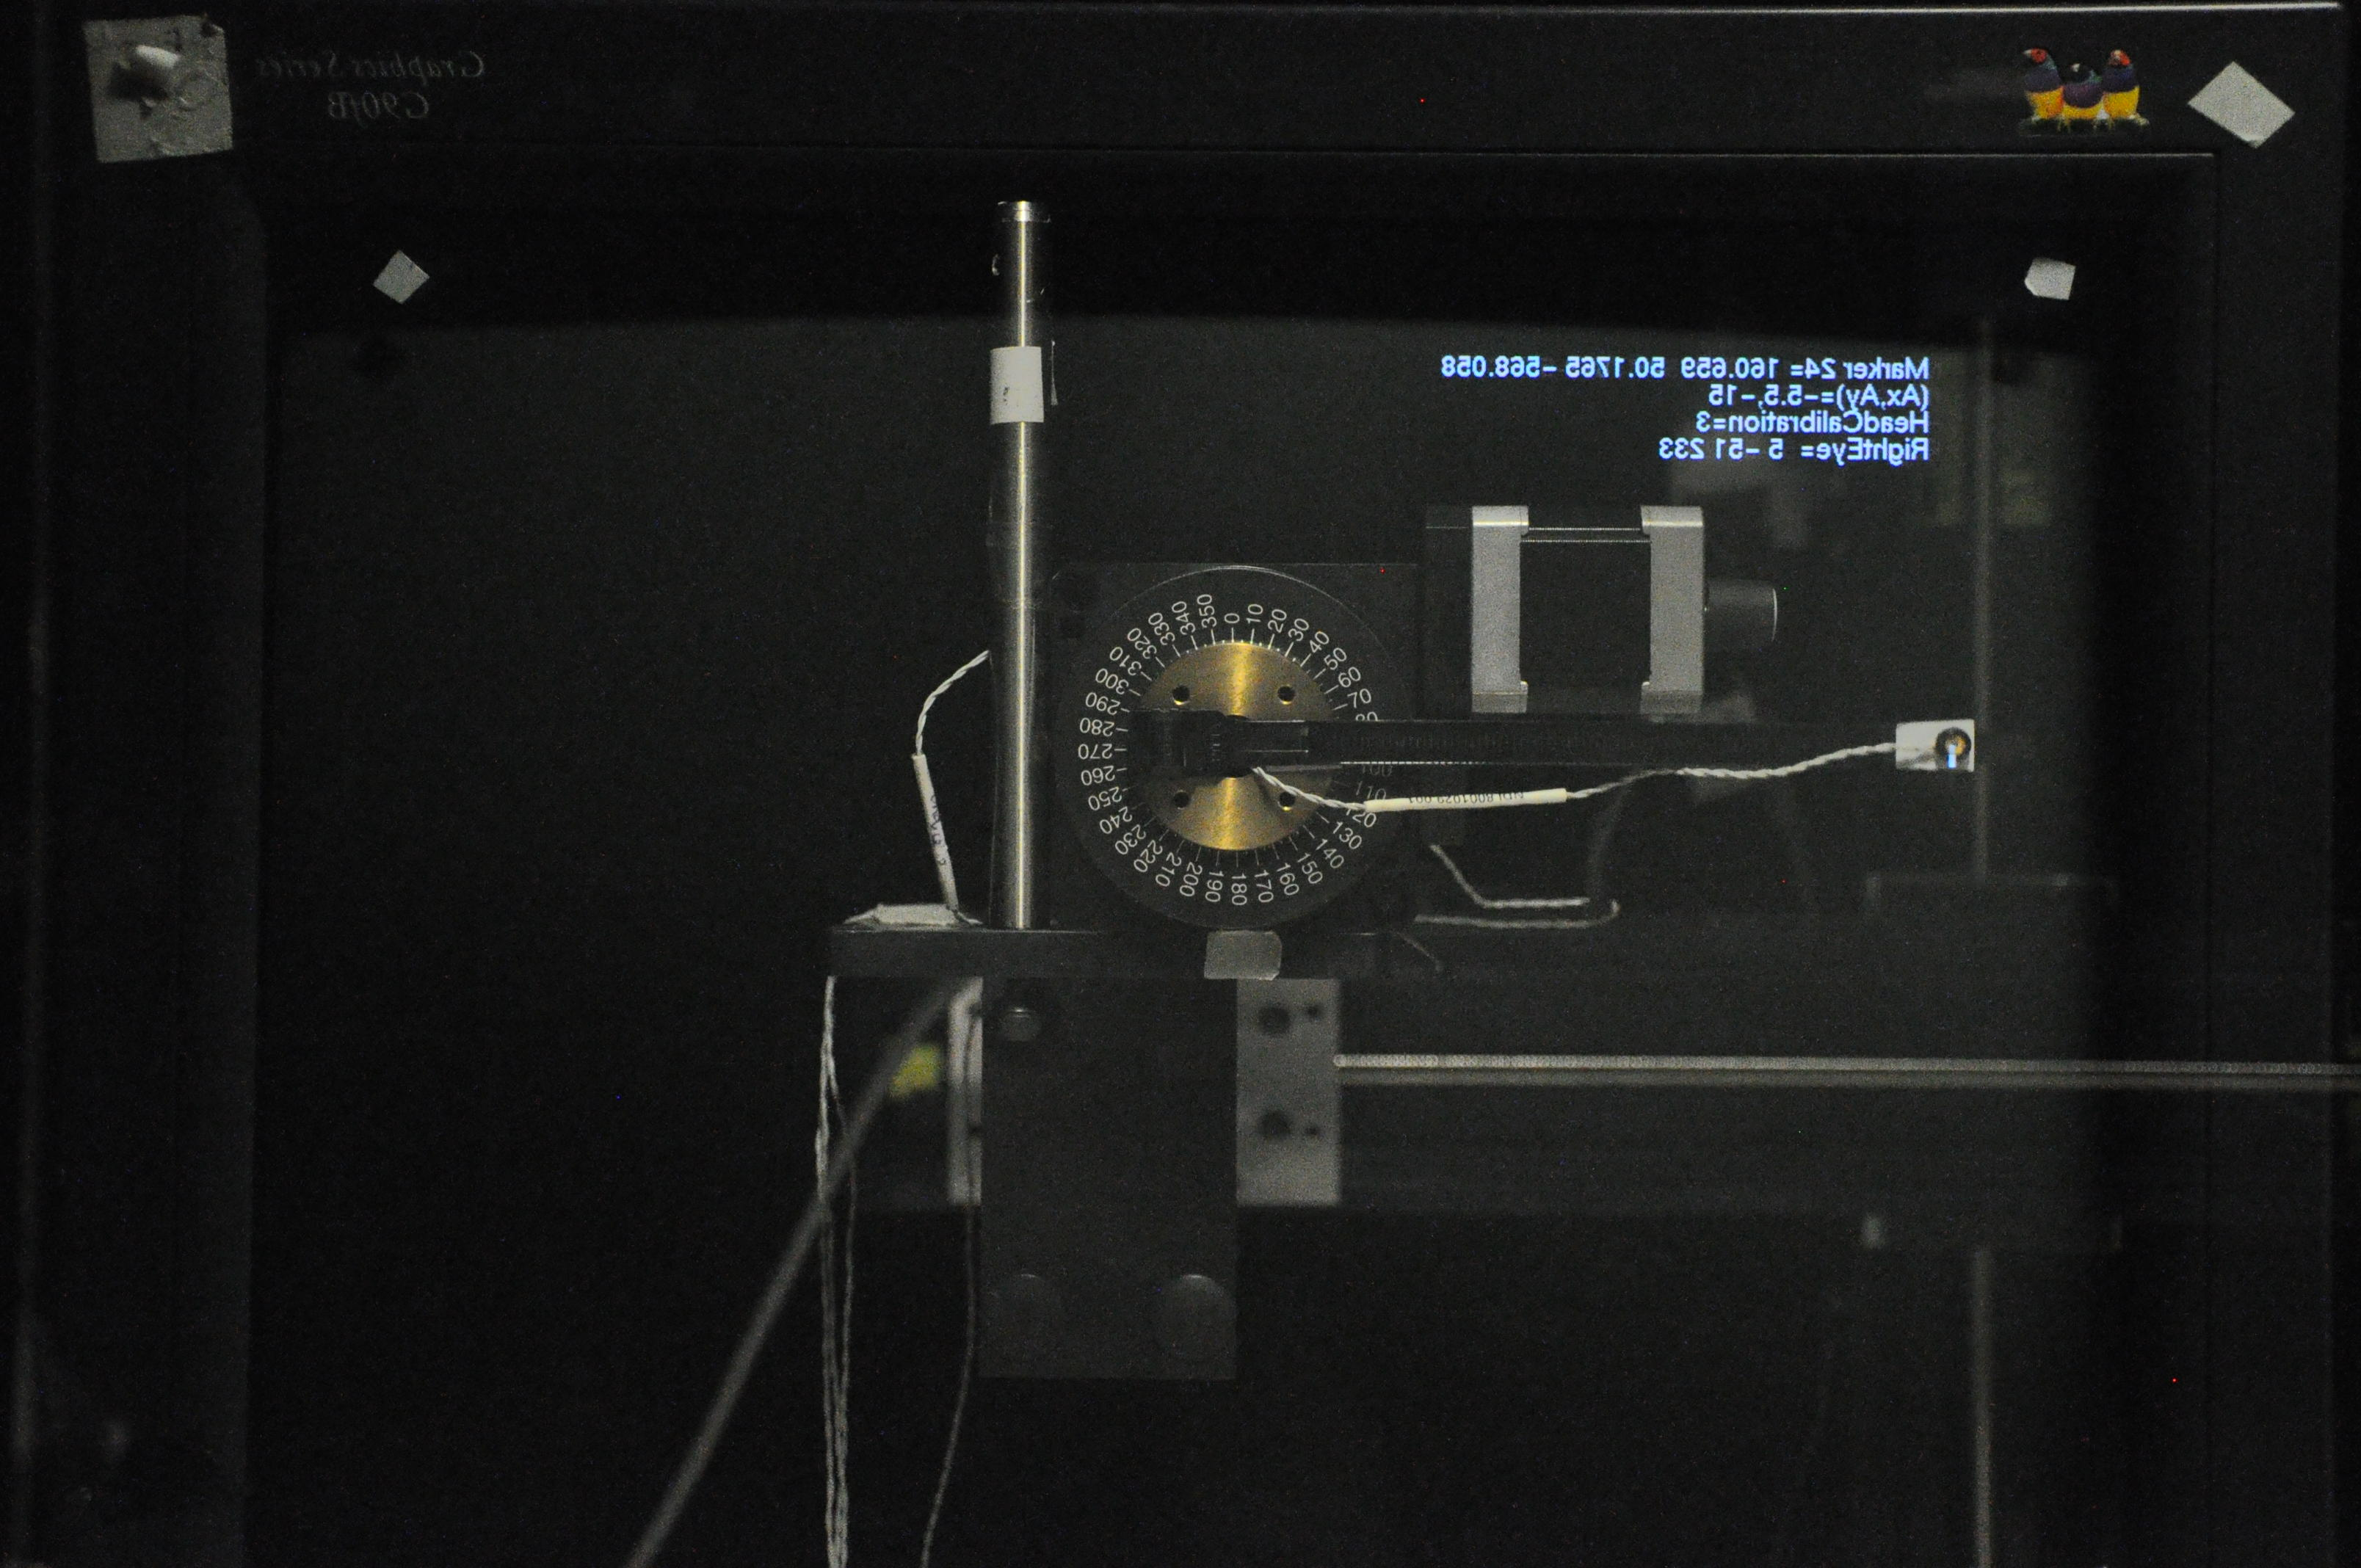
\includegraphics[width=0.75\textwidth]{images/test_1_simple/DSC_0138.JPG}
\caption{One of the photographs used for the computation}
\end{figure}

\begin{figure}[htb!]
\centering
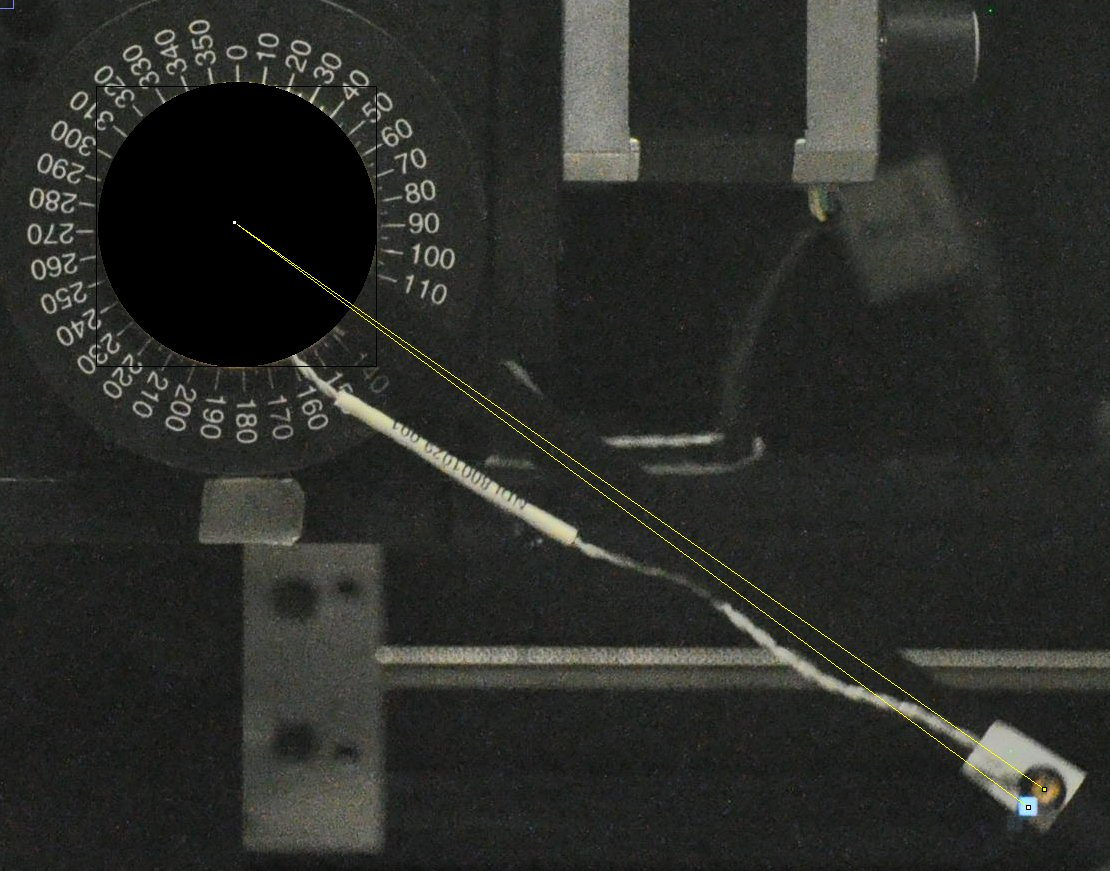
\includegraphics[width=0.75\textwidth]{images/measurement_method.jpg}
\caption{The method of measurement used in ImageJ}
\end{figure}
\clearpage

\section{Analysis}
We averaged the measures took at different time intervals.

\begin{figure}[htb!]
\centering
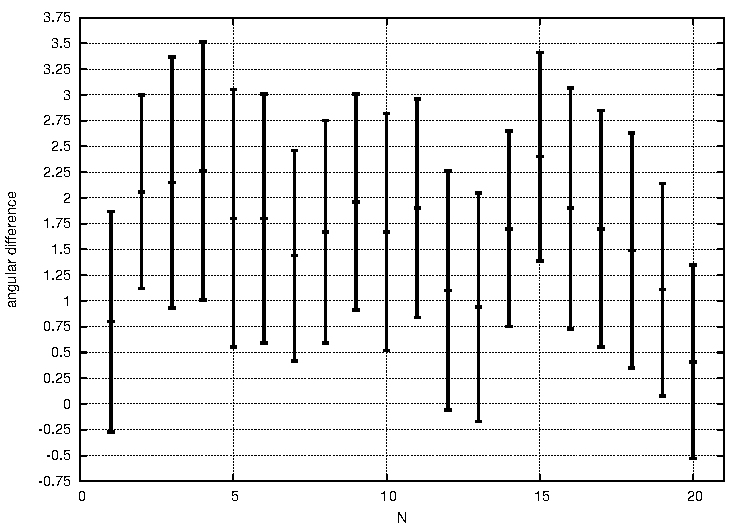
\includegraphics[width=1.0\textwidth]{data/angles_test_1.pdf}
\caption{Angular measures and their relative errorbars}
\end{figure}

The resulting average over $N=20$ observations of time-lags is $\left < \Delta t \right > = \left < \Delta \theta \right >/\omega \approx 0.027$ [s]. 
The resulting average over $N=20$ observations of time-lags error is $\left < \sigma_{\Delta t} \right > = \left < \Delta \theta \right >/\omega \approx 0.018$ [s]. 
See table (see \ref{tab:table_exp_1}).
\section{Analysis second experiment}
We repeated the experiment described before, with a heavier task. We were displaying a complex mesh with more than $10^6$ vertices, (see \ref{tab:table_exp2}) together with the dot and marker in order to check if the system is good also for more complex stimuli.

\begin{table}[htb!]\label{tab:table_exp2}
\centering
\begin{tabular}{|l|l|r|} \hline
$i$ & $\Delta \theta$ [deg] & $\sigma_{\Delta \theta}$ [deg]\\
\hline 
1 & 0.89 & 0.90 \\ \hline
2 & 1.48 & 1.17 \\ \hline
3 & 1.86 & 1.01 \\ \hline
4 & 1.86 & 1.01 \\ \hline
5 & 1.86 & 1.05 \\ \hline
6 & 2.16 & 1.01 \\ \hline
7 & 2.53 & 0.97 \\ \hline
8 & 2.43 & 1.05 \\ \hline
9 & 2.21 & 1.11 \\ \hline
10 & 2.03 & 1.06 \\
\hline
\end{tabular}
\begin{tabular}{|l|l|r|} \hline
$i$ & $\Delta \theta$ [deg] & $\sigma_{\Delta \theta}$ [deg]\\
\hline 
11 & 1.82 & 1.12 \\ \hline
12 & 1.60 & 0.97 \\ \hline
13 & 1.09 & 1.02 \\ \hline
14 & 1.38 & 1.10 \\ \hline
15 & 2.16 & 1.02 \\ \hline
16 & 1.21 & 1.23 \\ \hline
17 & 1.26 & 1.07 \\ \hline
18 & 1.52 & 1.10 \\ \hline
19 & 1.86 & 1.05 \\ \hline
20 & 1.57 & 1.01 \\
\hline
\end{tabular}
\caption{Table of data for experiment with complex mesh}
\end{table}

The resulting time-lag is $\left < \Delta t \right > = \left < \Delta \theta \right >/\omega \approx 0.029 \pm  0.074 $ [s].


\end{document}
